\chapter{Results}\label{ch:Results}

\subsection{Analysis}

\subsection{Software simulation}

\subsubsection{Jerk ramp}
CNO = 45

PLLBW =32
FLLBW = 10
76.135, std = 2.3549

PLLBW = 18
FLLBW = 1
128.26,std =  2.59 

PLLBW = 32
FLLBW = 0
131.6 std = 1.64

\begin{figure}[!htb] 
    \centering
    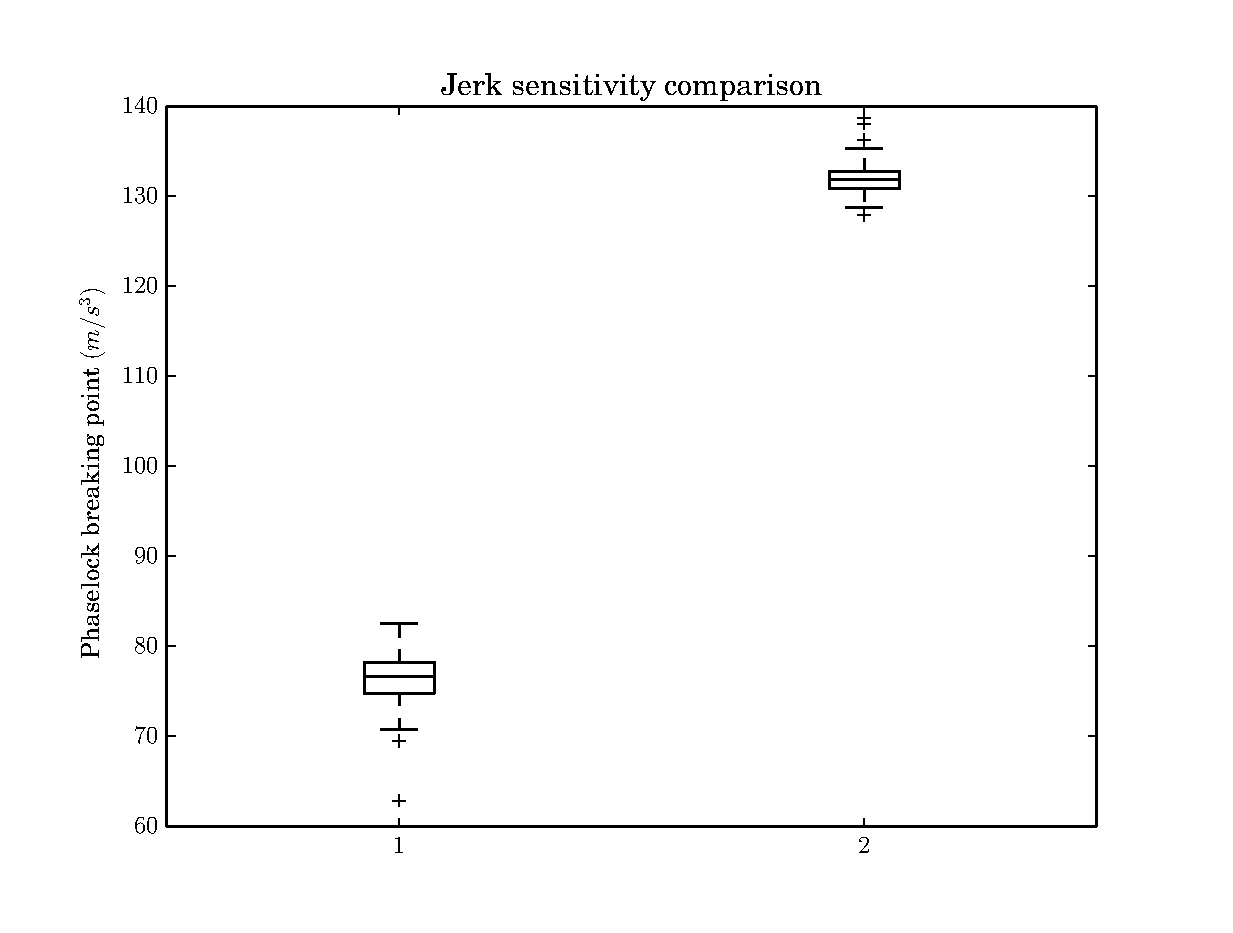
\includegraphics[width=1\textwidth]{mywork/BoxplotJerk.eps} 
    \caption{ 76.135, std = 2.3549 vs 131.6 std = 1.64}
    \label{fig:BoxplotJerk}
\end{figure}

\begin{figure}[!htb] 
    \centering
    \includegraphics[width=1\textwidth]{mywork/BoxplotPhaseJitter.eps} 
    \caption{5.77987052071 0.280738421289 vs 4.3143405835 0.0443823631819}
    \label{fig:BoxplotPhaseJitter}
\end{figure}

\subsubsection{HighG3}

\begin{table}[!htb]
\centering
\begin{tabular}{|l|l|l|}
\hline
\rowcolor[HTML]{C0C0C0} 
SVNUM & Lock time (\%) & Phase jitter (degrees) \\ \hline
0     & 99.9938868669  & 2.94532640253          \\ \hline
\rowcolor[HTML]{EFEFEF} 
1     & 99.993408762   & 2.94769915199          \\ \hline
3     & 99.9938868669  & 2.94919518101          \\ \hline
\rowcolor[HTML]{EFEFEF} 
6     & 99.9938868669  & 2.94102526044          \\ \hline
11    & 99.9938868669  & 2.94545139336          \\ \hline
\rowcolor[HTML]{EFEFEF} 
14    & 99.9923341049  & 2.95730497982          \\ \hline
16    & 99.9938868669  & 2.94859458495          \\ \hline
\rowcolor[HTML]{EFEFEF} 
18    & 99.9938868669  & 2.94407487114          \\ \hline
19    & 99.9938868669  & 2.94368018213          \\ \hline
\rowcolor[HTML]{EFEFEF} 
21    & 99.9446285568  & 3.11426406624          \\ \hline
22    & 99.9927007366  & 2.943947352            \\ \hline
\rowcolor[HTML]{EFEFEF} 
23    & 99.9932697205  & 2.95135953662          \\ \hline
25    & 97.5933488168  & 8.73693451462          \\ \hline
\rowcolor[HTML]{EFEFEF} 
31    & 99.9923357734  & 2.94442277494          \\ \hline
\end{tabular}

\caption{CNO = 48,PLLBW =32,FLL=0}
\label{my-label}
\end{table}


\begin{table}[!htb]
\centering
\begin{tabular}{|l|l|l|}
\hline
\rowcolor[HTML]{C0C0C0} 
SVNUM & Lock time (\%) & Phase jitter (degrees) \\ \hline
0     & 99.9938868669  & 4.10539966514          \\ \hline
\rowcolor[HTML]{EFEFEF} 
1     & 99.993408762   & 4.10334714077          \\ \hline
3     & 99.9938868669  & 4.1079353616           \\ \hline
\rowcolor[HTML]{EFEFEF} 
6     & 99.9938868669  & 4.1031216192           \\ \hline
11    & 99.9938868669  & 4.11852598123          \\ \hline
\rowcolor[HTML]{EFEFEF} 
14    & 99.9923341049  & 4.12708223476          \\ \hline
16    & 99.9938868669  & 4.10894682099          \\ \hline
\rowcolor[HTML]{EFEFEF} 
18    & 99.9938868669  & 4.13975681239          \\ \hline
19    & 99.9938868669  & 4.12705835872          \\ \hline
\rowcolor[HTML]{EFEFEF} 
21    & 99.9446285568  & 4.17746647598          \\ \hline
22    & 99.9938868669  & 4.13428070614          \\ \hline
\rowcolor[HTML]{EFEFEF} 
23    & 99.9917629415  & 4.13411130351          \\ \hline
25    & 97.5873761308  & 9.22106274762          \\ \hline
\rowcolor[HTML]{EFEFEF} 
31    & 99.9938868669  & 4.11195994528          \\ \hline
\end{tabular}
\caption{CNO = 48,PLLBW =32,FLL=10}
\label{my-label}
\end{table}



\begin{table}[!htb]
\centering
\begin{tabular}{|l|l|l|}
\hline
\rowcolor[HTML]{C0C0C0} 
SVNUM & Lock time (\%) & Phase jitter (degrees) \\ \hline
0     & 99.9938868669  & 5.85150590292          \\ \hline
\rowcolor[HTML]{EFEFEF} 
1     & 99.9925233718  & 5.8678088226           \\ \hline
3     & 99.9923357734  & 5.8552560291           \\ \hline
\rowcolor[HTML]{EFEFEF} 
6     & 99.9938868669  & 5.8622244764           \\ \hline
11    & 99.9936131445  & 5.86698613227          \\ \hline
\rowcolor[HTML]{EFEFEF} 
14    & 99.9923341049  & 5.85976998793          \\ \hline
16    & 99.9938868669  & 5.86700880521          \\ \hline
\rowcolor[HTML]{EFEFEF} 
18    & 99.9938868669  & 5.86355144123          \\ \hline
19    & 99.9919708102  & 5.88993271515          \\ \hline
\rowcolor[HTML]{EFEFEF} 
21    & 99.9446285568  & 5.89517718701          \\ \hline
22    & 99.9936131445  & 5.86991081749          \\ \hline
\rowcolor[HTML]{EFEFEF} 
23    & 99.9911602299  & 5.86469530411          \\ \hline
25    & 59.8254951783  & 33.3414856714          \\ \hline
\rowcolor[HTML]{EFEFEF} 
31    & 99.9938868669  & 5.86106301871          \\ \hline
\end{tabular}
\caption{CNO = 42,PLLBW =32,FLL=0}
\label{my-label}
\end{table}

\begin{table}[]
\centering
\begin{tabular}{|l|l|l|}
\hline
\rowcolor[HTML]{C0C0C0} 
SVNUM & Lock time (\%) & Phase jitter (degrees) \\ \hline
0     & 99.9916058471  & 8.22732333217          \\ \hline
\rowcolor[HTML]{EFEFEF} 
1     & 99.9923266185  & 8.22539162245          \\ \hline
3     & 99.9927007366  & 8.21735356196          \\ \hline
\rowcolor[HTML]{EFEFEF} 
6     & 99.9938868669  & 8.20734346342          \\ \hline
11    & 99.9921532918  & 8.21523460807          \\ \hline
\rowcolor[HTML]{EFEFEF} 
14    & 99.9923341049  & 8.21732089483          \\ \hline
16    & 99.9927007366  & 8.2150754949           \\ \hline
\rowcolor[HTML]{EFEFEF} 
18    & 99.9938868669  & 8.2076813485           \\ \hline
19    & 99.9923357734  & 8.2395476463           \\ \hline
\rowcolor[HTML]{EFEFEF} 
21    & 99.9371906017  & 8.25529372615          \\ \hline
22    & 99.9928832182  & 8.22342517274          \\ \hline
\rowcolor[HTML]{EFEFEF} 
23    & 99.9917629415  & 8.22683126791          \\ \hline
25    & 43.5826901319  & 39.6450990098          \\ \hline
\rowcolor[HTML]{EFEFEF} 
31    & 99.9938868669  & 8.2146771752           \\ \hline
\end{tabular}
\caption{CNO = 42,PLLBW =32,FLL=10}
\label{my-label}
\end{table}

\subsection{Hardware simulation}

\subsubsection{HighG3}

\subsection{Discussion}




